\documentclass[11pt, oneside]{article}   	% use "amsart" instead of "article" for AMSLaTeX format
\usepackage{geometry}                		% See geometry.pdf to learn the layout options. There are lots.
\geometry{letterpaper}                   		% ... or a4paper or a5paper or ... 
%\geometry{landscape}                		% Activate for for rotated page geometry
%\usepackage[parfill]{parskip}    		% Activate to begin paragraphs with an empty line rather than an indent
\usepackage{graphicx}				% Use pdf, png, jpg, or eps� with pdflatex; use eps in DVI mode
								% TeX will automatically convert eps --> pdf in pdflatex		
\usepackage{amssymb}
\usepackage{amsmath}
\usepackage{parskip}

\title{Don't be irrational, $e$}
%\author{The Author}
\date{}							% Activate to display a given date or no date

\graphicspath{{/Users/telliott_admin/Dropbox/Tex/png/}}
\begin{document}

\maketitle
%\section{}
% \subsection*{R code}
% \begin{lstlisting}  \end{lstlisting}
% \begin{center} 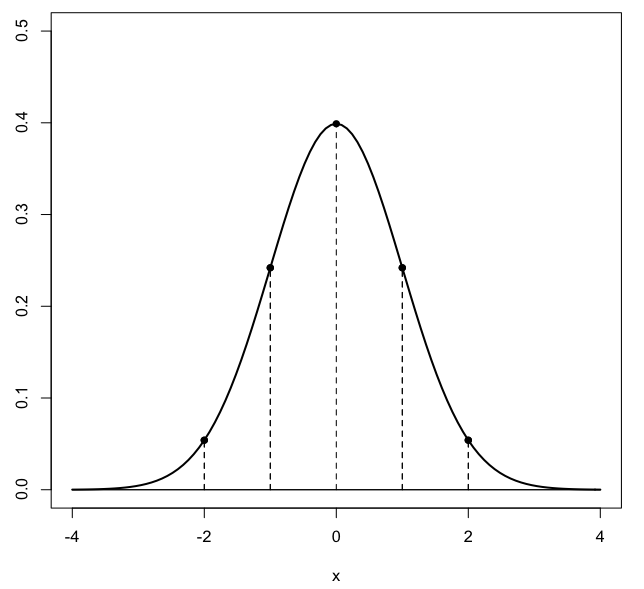
\includegraphics [scale=0.4] {gauss3.png} \end{center}
% \begin{bmatrix} a  &  b \\ c  &  d \end{bmatrix}
% \bigg |_
\Large
I found a nice proof of the irrationality of $e$ in the calculus text by Courant and Robbins.  It is a proof by contradiction.  We start by assuming that $e$ is rational.
\[ e = \frac{p}{q}, \ \  p,q \in \mathbb{N} \]
We make use of the infinite series representation of $e$
\[ e = 1 + 1 + \frac{1}{2!}  + \frac{1}{3!} + \frac{1}{4!} + \cdots \]
From this, it is obvious that $e > 2$.  If you're interested, there is a proof that $e < 3$ in the book.  

% But I will just say that if $e=p/q$ with $p$ and $q$ integers, and $e>2$, then $q>1$ so $q>=2$.
Equating the series representation to the rational fraction $p/q$:
\[ \frac{p}{q} = 1 + 1 + \frac{1}{2!}  + \frac{1}{3!} + \frac{1}{4!} + \cdots \]
Multiply both sides by $q!$.  For the left-hand side, we have 
\[ e \ q! = \frac{p}{q} \ q! = p (q-1)! \]
We won't need to do anything more with this, but note that since $e\ q!$ is equal to $p (q-1)!$, we can see that the left-hand side, $e\ q!$, is clearly an integer.
Therefore, the right-hand side must also be an integer.  This is the series
\[ q! + q! + \frac{q!}{2!}  + \frac{q!}{3!}  + \cdots + \frac{q!}{(q-1)!} + \frac{q!}{q!} + \frac{q!}{(q+1)!} + \cdots \]
Now, 
$q!$ is obviously an integer. And for every integer $k < q$, $k!$ divides $q!$ evenly 
\[ \frac{q!}{k!} = q \times (q-1) \times (q-2) \cdots \times (q-k+1) \]
In our series
\[ q! + q! + \frac{q!}{2!}  + \frac{q!}{3!}  + \cdots + \frac{q!}{(q-1)!} + \frac{q!}{q!} + \frac{q!}{(q+1)!} + \cdots \]
all the terms to the left of $q!/(q-1)!$ are integers, as is $q!/(q-1)! = q$ and $q!/q! = 1$.  
\vspace{2 mm}

So now our concern is with the fractions that follow.  We will show that these sum up to something less than $1$.  We have
\[ \frac{1}{(q+1)} + \frac{1}{(q+1)(q+2)} + \frac{1}{(q+1)(q+2)(q+3)} + \cdots \]
Since $q >= 2$
\[ \frac{1}{(q+1)} <= \frac{1}{3} \]
\[ \frac{1}{(q+1)(q+2)} <= (\frac{1}{3})^2 \]
and so on, and the entire remaining series of fractions is less than or equal to
\[ \frac{1}{3} + (\frac{1}{3})^2 + (\frac{1}{3})^3 + \cdots \]
This is the geometric series with $r = 1/3$ and first term equal to r, and the sum is known to be
\[ \frac{1}{3} ( 1 / (1-\frac{1}{3}) ) = \frac{1}{2} \]
Since the right-hand side is equal to an integer plus something "less than or equal to $\frac{1}{2}$", it is not an integer, and cannot be equal to the left-hand side, which is equal to an integer.  We have reached a contradiction.  Therefore $e$ cannot be equal to $p/q$, for $p,q \in \mathbb{N}$.


\end{document}  